% answers.tex —— 2007 年·普通高等学校招生考试·湖北卷·文科 · 参考答案与详细解析片段
% 由 tools/generate_projects.py 依来源总账自 2007/2007_数学真题_湖北文_试题.md + 2007/2007_数学真题_湖北文_解析正文.md + 2007/2007_数学真题_湖北文_答案要点.md 生成，勿手改（改源 MD 后重跑）


\begin{gktip}
固定候选 PDF 仅含题面，无答案、解析和评分标准，原卷亦未标注分值；以下为非官方编者独立推导，官方答案字段为空。来源发布者、出版者、版次与官方身份均未核。
\end{gktip}

\begin{answer}
\gksolhead{1}{}

\textbf{题目}：

$\tan690^\circ$ 的值为（　）

（A）$-\dfrac{\sqrt3}{3}$

（B）$\dfrac{\sqrt3}{3}$

（C）$\sqrt3$

（D）$-\sqrt3$

\Needspace{4\baselineskip}
\textbf{解析}

\nopagebreak[4]
\[\tan690^\circ=\tan(690^\circ-720^\circ)=\tan(-30^\circ)=-\frac{\sqrt3}{3}.\]

\gkanswer{答案：A。}

\end{answer}
\begin{answer}
\gksolhead{2}{}

\textbf{题目}：

如果 $U=\{x\mid x$ 是小于 $9$ 的正整数$\}$，$A=\{1,2,3,4\}$，$B=\{3,4,5,6\}$，那么 $\complement_UA\cap\complement_UB=$（　）

（A）$\{1,2\}$

（B）$\{3,4\}$

（C）$\{5,6\}$

（D）$\{7,8\}$

\Needspace{4\baselineskip}
\textbf{解析}

\Needspace{5\baselineskip}
$U=\{1,2,\ldots,8\}$，$\complement_UA=\{5,6,7,8\}$，$\complement_UB=\{1,2,7,8\}$，故

\nopagebreak[4]
\[\complement_UA\cap\complement_UB=\{7,8\}.\]

\gkanswer{答案：D。}

\end{answer}
\begin{answer}
\gksolhead{3}{}

\textbf{题目}：

如果 $\left(3x^2-\dfrac{2}{x^3}\right)^n$ 的展开式中含有非零常数项，则正整数 $n$ 的最小值为（　）

（A）$10$

（B）$6$

（C）$5$

（D）$3$

\Needspace{4\baselineskip}
\textbf{解析}

\Needspace{5\baselineskip}
通项

\nopagebreak[4]
\[\mathrm C_n^k(3x^2)^{n-k}\left(-\frac2{x^3}\right)^k\]

的指数为 $2(n-k)-3k=2n-5k$。令其为零，$k=\dfrac{2n}{5}$，故 $n$ 为 $5$ 的倍数，最小 $n=5$（此时 $k=2$）。

\gkanswer{答案：C。}

\end{answer}
\begin{answer}
\gksolhead{4}{}

\textbf{题目}：

函数 $y=\dfrac{2^x+1}{2^x-1}$（$x<0$）的反函数是（　）

（A）$y=\log_2\dfrac{x+1}{x-1}$（$x<-1$）

（B）$y=\log_2\dfrac{x+1}{x-1}$（$x>1$）

（C）$y=\log_2\dfrac{x-1}{x+1}$（$x<-1$）

（D）$y=\log_2\dfrac{x-1}{x+1}$（$x>1$）

\Needspace{4\baselineskip}
\textbf{解析}

\Needspace{5\baselineskip}
令 $y=\dfrac{2^x+1}{2^x-1}$，解得

\nopagebreak[4]
\[2^x=\frac{y+1}{y-1}.\]

\Needspace{5\baselineskip}
由 $x<0$ 得 $0<2^x<1$，故

\nopagebreak[4]
\[0<\frac{y+1}{y-1}<1,\]

\Needspace{5\baselineskip}
解得 $y<-1$。交换 $x$，$y$ 得反函数

\nopagebreak[4]
\[y=\log_2\frac{x+1}{x-1}\quad(x<-1).\]

\gkanswer{答案：A。}

\end{answer}
\begin{answer}
\gksolhead{5}{}

\textbf{题目}：

在棱长为 $1$ 的正方体 $ABCD-A_1B_1C_1D_1$ 中，$E$，$F$ 分别为棱 $AA_1$，$BB_1$ 的中点，$G$ 为棱 $A_1B_1$ 上的一点，且 $A_1G=\lambda$（$0\leqslant\lambda\leqslant1$），则点 $G$ 到平面 $D_1EF$ 的距离为（　）
\nopagebreak[4]
\begin{center}% 2007 年湖北卷文科第 5 题：正方体 ABCD-A1B1C1D1，E、F 为 AA1、BB1 中点，
%   G 在 A1B1 上，平面 D1EF 与 G 的位置。
% 来源 PDF：gaokaomath-src/普通高考/2007/2007湖北文.pdf
% SHA-256：290a153da24ec0f3a3abb8bb916d9b7e06d203d3ef5bd7bb221c93f7f1b1cacb
% 原页：2007湖北文.pdf 第 1 页（A3 三栏）第 1 栏，书页码 377。
% 重绘依据：按原页正方体斜投影、E/F/G 与平面 D1EF 的虚实线重绘。
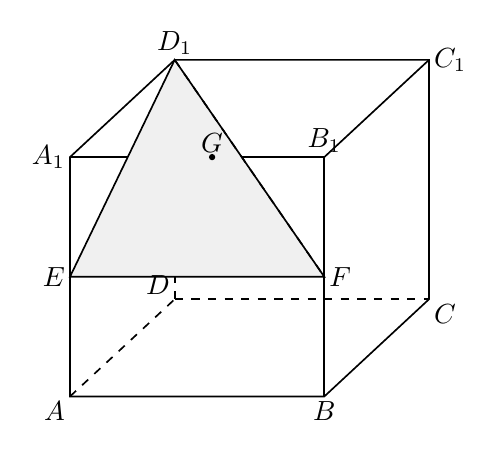
\begin{tikzpicture}[scale=0.95, semithick,
  every node/.style={inner sep=1.5pt}]
  \coordinate (A)  at (0,0);
  \coordinate (B)  at (3.4,0);
  \coordinate (C)  at (4.8,1.3);
  \coordinate (D)  at (1.4,1.3);
  \coordinate (A1) at (0,3.2);
  \coordinate (B1) at (3.4,3.2);
  \coordinate (C1) at (4.8,4.5);
  \coordinate (D1) at (1.4,4.5);
  \coordinate (E)  at (0,1.6);
  \coordinate (F)  at (3.4,1.6);
  \coordinate (G)  at (1.9,3.2);

  \draw[dashed] (A) -- (D);
  \draw[dashed] (D) -- (C);
  \draw[dashed] (D) -- (D1);
  \draw (A) -- (B) -- (C) -- (C1) -- (D1) -- (A1) -- cycle;
  \draw (A) -- (A1); \draw (B) -- (B1); \draw (C) -- (C1);
  \draw (A1) -- (B1); \draw (B1) -- (C1);
  % 平面 D1EF
  \fill[gray!12] (D1) -- (E) -- (F) -- cycle;
  \draw (D1) -- (E) -- (F) -- cycle;
  \draw[dashed] (D1) -- (F);
  \fill (G) circle (1.2pt);

  \node[below left] at (A) {$A$};
  \node[below] at (B) {$B$};
  \node[below right] at (C) {$C$};
  \node[above left] at (D) {$D$};
  \node[left] at (A1) {$A_1$};
  \node[above] at (B1) {$B_1$};
  \node[right] at (C1) {$C_1$};
  \node[above] at (D1) {$D_1$};
  \node[left] at (E) {$E$};
  \node[right] at (F) {$F$};
  \node[above] at (G) {$G$};
\end{tikzpicture}
\end{center}
\nopagebreak[4]
（A）$\sqrt3$

（B）$\dfrac{\sqrt2}{2}$

（C）$\dfrac{\sqrt2\lambda}{2}$

（D）$\dfrac{\sqrt5}{5}$

\Needspace{4\baselineskip}
\textbf{解析}

\Needspace{5\baselineskip}
以 $A$ 为原点，$AB$，$AD$，$AA_1$ 为 $x$，$y$，$z$ 轴：

\nopagebreak[4]
\[E\left(0,0,\frac12\right),\quad F\left(1,0,\frac12\right),\quad D_1(0,1,1),\quad G(\lambda,0,1).\]

\Needspace{5\baselineskip}
平面 $D_1EF$ 的法向量为 $(0,-1,2)$，平面方程

\nopagebreak[4]
\[-y+2z-1=0.\]

\Needspace{5\baselineskip}
$G$ 到平面的距离

\nopagebreak[4]
\[d=\frac{|0-0+2-1|}{\sqrt{0+1+4}}=\frac1{\sqrt5}=\frac{\sqrt5}{5},\]

与 $\lambda$ 无关。

\gkanswer{答案：D。}

\end{answer}
\begin{answer}
\gksolhead{6}{}

\textbf{题目}：

为了了解某学校学生的身体发育情况，抽查了该校 $100$ 名高中男生的体重情况，根据所得数据画出样本的频率分布直方图如图所示。根据此图，估计该校 $2000$ 名高中男生中体重大于 $70.5$ 公斤的人数为（　）
\nopagebreak[4]
\begin{center}% 2007 年湖北卷文科第 6 题：100 名男生体重的频率分布直方图。
%   组距 2 kg，横轴 52.5—76.5 kg，纵轴「频率/组距」0.01—0.08。
% 来源 PDF：gaokaomath-src/普通高考/2007/2007湖北文.pdf
% SHA-256：290a153da24ec0f3a3abb8bb916d9b7e06d203d3ef5bd7bb221c93f7f1b1cacb
% 原页：2007湖北文.pdf 第 1 页（A3 三栏）第 1 栏，书页码 377。
% 重绘依据：按原页 12 个等宽柱与纵轴刻度重绘，柱高按原图读取。
\begin{tikzpicture}[x=1.0cm, y=70cm, semithick,
  every node/.style={inner sep=1pt, font=\scriptsize}]
  \draw[->,>=stealth] (0,0) -- (12.8,0) node[right] {体重 (kg)};
  \draw[->,>=stealth] (0,0) -- (0,0.09) node[above] {频率/组距};

  \foreach \i/\h in {0/0.01,1/0.01,2/0.02,3/0.05,4/0.06,5/0.07,
                     6/0.08,7/0.065,8/0.05,9/0.04,10/0.03,11/0.02} {
    \draw (\i,0) rectangle (\i+1,\h);
  }

  \foreach \y in {0.01,0.02,0.03,0.04,0.05,0.06,0.07,0.08} {
    \draw (0,\y) -- (-0.12,\y);
    \node[left] at (0,\y) {\y};
  }
  \node[below left] at (0,0) {$O$};
  \foreach \i in {1,...,12} {
    \draw (\i,0) -- (\i,-0.0015);
    \node[below] at (\i,0) {\the\numexpr 52+2*\i\relax.5};
  }
\end{tikzpicture}
\end{center}
\nopagebreak[4]
（A）$300$

（B）$360$

（C）$420$

（D）$450$

\Needspace{4\baselineskip}
\textbf{解析}

\Needspace{5\baselineskip}
$70.5$ 公斤以上的三个组为 $[70.5,72.5)$，$[72.5,74.5)$，$[74.5,76.5)$，频率分别为

\nopagebreak[4]
\[0.04\times2=0.08,\quad0.03\times2=0.06,\quad0.02\times2=0.04,\]

\Needspace{5\baselineskip}
合计 $0.18$。故人数约为

\nopagebreak[4]
\[2000\times0.18=360.\]

\gkanswer{答案：B。}

\end{answer}
\begin{answer}
\gksolhead{7}{}

\textbf{题目}：

将 $5$ 本不同的书全发给 $4$ 名同学，每名同学至少有一本书的概率是（　）

（A）$\dfrac{15}{64}$

（B）$\dfrac{15}{128}$

（C）$\dfrac{24}{125}$

（D）$\dfrac{48}{125}$

\Needspace{4\baselineskip}
\textbf{解析}

\Needspace{5\baselineskip}
$5$ 本书分给 $4$ 人且每人至少一本，人数分配为 $2,1,1,1$。分法数

\nopagebreak[4]
\[\mathrm C_5^2\cdot4!=240,\]

\Needspace{5\baselineskip}
总分法 $4^5=1024$，概率

\nopagebreak[4]
\[\frac{240}{1024}=\frac{15}{64}.\]

\gkanswer{答案：A。}

\end{answer}
\begin{answer}
\gksolhead{8}{}

\textbf{题目}：

由直线 $y=x+1$ 上的一点向圆 $(x-3)^2+y^2=1$ 引切线，则切线长的最小值为（　）

（A）$1$

（B）$2\sqrt2$

（C）$\sqrt7$

（D）$3$

\Needspace{4\baselineskip}
\textbf{解析}

\Needspace{5\baselineskip}
圆心 $(3,0)$ 到直线 $x-y+1=0$ 的距离为

\nopagebreak[4]
\[d=\frac{|3-0+1|}{\sqrt2}=2\sqrt2.\]

\Needspace{5\baselineskip}
切线长

\nopagebreak[4]
\[\sqrt{d^2-r^2}=\sqrt{8-1}=\sqrt7.\]

\gkanswer{答案：C。}

\end{answer}
\begin{answer}
\gksolhead{9}{}

\textbf{题目}：

设 $\boldsymbol a=(4,3)$，$\boldsymbol a$ 在 $\boldsymbol b$ 上的投影为 $\dfrac{5\sqrt2}{2}$，$\boldsymbol b$ 在 $x$ 轴上的投影为 $2$，且 $|\boldsymbol b|\leqslant14$，则 $\boldsymbol b$ 为（　）

（A）$(2,14)$

（B）$\left(2,-\dfrac27\right)$

（C）$\left(-2,\dfrac27\right)$

（D）$(2,8)$

\Needspace{4\baselineskip}
\textbf{解析}

\Needspace{5\baselineskip}
设 $\boldsymbol b=(2,y)$（$x$ 轴投影为 $2$）。由投影公式

\nopagebreak[4]
\[\frac{|\boldsymbol a\cdot\boldsymbol b|}{|\boldsymbol b|}
=\frac{|8+3y|}{\sqrt{4+y^2}}=\frac{5\sqrt2}{2}.\]

\Needspace{5\baselineskip}
平方整理：

\nopagebreak[4]
\[2(64+48y+9y^2)=25(4+y^2),\]

\nopagebreak[4]
\[7y^2-96y-28=0,\]

\Needspace{5\baselineskip}
解得 $y=14$ 或 $y=-\dfrac27$。$y=14$ 时 $|\boldsymbol b|=\sqrt{200}>14$，舍去。故

\nopagebreak[4]
\[\boldsymbol b=\left(2,-\frac27\right).\]

\gkanswer{答案：B。}

\end{answer}
\begin{answer}
\gksolhead{10}{}

\textbf{题目}：

已知 $p$ 是 $r$ 的充分条件而不是必要条件，$q$ 是 $r$ 的充分条件，$s$ 是 $r$ 的必要条件，$q$ 是 $s$ 的必要条件，现有下列命题：

① $s$ 是 $q$ 的充要条件；

② $p$ 是 $q$ 的充分条件而不是必要条件；

③ $r$ 是 $q$ 的必要条件而不是充分条件；

④ $\neg p$ 是 $\neg s$ 的必要条件而不是充分条件；

⑤ $r$ 是 $s$ 的充分条件而不是必要条件。

则正确命题的序号是（　）

（A）①④⑤

（B）①②④

（C）②③⑤

（D）②④⑤

\Needspace{4\baselineskip}
\textbf{解析}

\Needspace{5\baselineskip}
由条件：$p\Rightarrow r$，$r\nRightarrow p$；$q\Rightarrow r$；$r\Rightarrow s$；$s\Rightarrow q$。于是

\nopagebreak[4]
\[r\Leftrightarrow s\Leftrightarrow q,\qquad p\Rightarrow q.\]

① $s$ 与 $q$ 等价，真；② $p\Rightarrow q$ 且 $q\nRightarrow p$，真；③ $r$ 与 $q$ 等价，故“必要而不充分”假；④ $p\Rightarrow s$，故 $\neg s\Rightarrow\neg p$，且反之不成立，真；⑤ $r$ 与 $s$ 等价，假。

正确的是①②④。

\gkanswer{答案：B。}

\end{answer}
\begin{answer}
\gksolhead{11}{}

\textbf{题目}：

设变量 $x$，$y$ 满足约束条件 $\begin{cases}x-y+3\geqslant0,\\ x+y\geqslant0,\\ -2\leqslant x\leqslant3,\end{cases}$ 则目标函数 $2x+y$ 的最小值为\gkblank{}。

\Needspace{4\baselineskip}
\textbf{解析}

\Needspace{5\baselineskip}
可行域的三个顶点为 $(-2,1)$，$(-2,2)$，$(3,-3)$（另两个交点不在约束内）。计算

\nopagebreak[4]
\[2x+y:\quad (-2,1)\to-3,\quad(-2,2)\to-2,\quad(3,-3)\to3.\]

最小值为 $-3$。

\gkanswer{答案：$-3$。}

\end{answer}
\begin{answer}
\gksolhead{12}{}

\textbf{题目}：

过双曲线 $\dfrac{x^2}{4}-\dfrac{y^2}{3}=1$ 左焦点 $F_1$ 的直线交双曲线的左支于 $M$，$N$ 两点，$F_2$ 为其右焦点，则 $|MF_2|+|NF_2|-|MN|$ 的值为\gkblank{}。

\Needspace{4\baselineskip}
\textbf{解析}

\Needspace{5\baselineskip}
$M$，$N$ 在左支上，由双曲线定义

\nopagebreak[4]
\[|MF_2|-|MF_1|=2a=4,\qquad |NF_2|-|NF_1|=4.\]

\Needspace{5\baselineskip}
$F_1$ 在线段 $MN$ 上，故 $|MF_1|+|NF_1|=|MN|$。相加得

\nopagebreak[4]
\[|MF_2|+|NF_2|-|MN|=8.\]

\gkanswer{答案：$8$。}

\end{answer}
\begin{answer}
\gksolhead{13}{}

\textbf{题目}：

已知函数 $y=f(x)$ 的图象在点 $M(1,f(1))$ 处的切线方程是 $y=\dfrac12x+2$，则 $f(1)+f'(1)=$\gkblank{}。

\Needspace{4\baselineskip}
\textbf{解析}

\Needspace{5\baselineskip}
切线 $y=\dfrac12x+2$ 在 $x=1$ 处给出

\nopagebreak[4]
\[f(1)=\frac12+2=\frac52,\qquad f'(1)=\frac12.\]

\Needspace{5\baselineskip}
故

\nopagebreak[4]
\[f(1)+f'(1)=3.\]

\gkanswer{答案：$3$。}

\end{answer}
\begin{answer}
\gksolhead{14}{}

\textbf{题目}：

某男运动员在三分线投球的命中率是 $\dfrac12$，他投球 $10$ 次，恰好投进 $3$ 个球的概率为\gkblank{}。（用数值作答）

\Needspace{4\baselineskip}
\textbf{解析}

\nopagebreak[4]
\[P=\mathrm C_{10}^3\left(\frac12\right)^{10}=\frac{120}{1024}=\frac{15}{128}.\]

\gkanswer{答案：$\dfrac{15}{128}$。}

\end{answer}
\begin{answer}
\gksolhead{15}{}

\textbf{题目}：

为了预防流感，某学校对教室用药熏消毒法进行消毒。已知药物释放过程中，室内每立方米空气中的含药量 $y$（毫克）与时间 $t$（小时）成正比；药物释放完毕后，$y$ 与 $t$ 的函数关系式为 $y=\left(\dfrac1{16}\right)^{t-a}$（$a$ 为常数），如图所示。

（1）从药物释放开始，每立方米空气中的含药量 $y$（毫克）与时间 $t$（小时）之间的函数关系式为\gkblank{}；

（2）据测定，当空气中每立方米的含药量降低到 $0.25$ 毫克以下时，学生方可进教室，那么药物释放开始，至少需要经过\gkblank{}小时后，学生才能回到教室。
\nopagebreak[4]
\begin{center}% 2007 年湖北卷文科第 15 题：药物释放过程中含药量 y 与时间 t 的关系图。
%   0—0.1 小时线性上升至 1 毫克，0.1 小时后按 (1/16)^(t-a) 衰减。
% 来源 PDF：gaokaomath-src/普通高考/2007/2007湖北文.pdf
% SHA-256：290a153da24ec0f3a3abb8bb916d9b7e06d203d3ef5bd7bb221c93f7f1b1cacb
% 原页：2007湖北文.pdf 第 1 页（A3 三栏）第 3 栏，书页码 377。
% 重绘依据：按原页折线—曲线衔接点 (0.1,1) 与衰减趋势重绘。
\begin{tikzpicture}[x=4.2cm, y=1.5cm, semithick,
  every node/.style={inner sep=1pt}]
  \draw[->,>=stealth] (0,0) -- (1.25,0) node[right] {$t$ (小时)};
  \draw[->,>=stealth] (0,0) -- (0,1.25) node[above] {$y$ (毫克)};
  \node[below left] at (0,0) {$O$};
  \draw (0,0) -- (0.1,1);
  \draw[domain=0.1:1.15,samples=100] plot (\x,{(1/16)^(\x-0.1)});
  \draw[dashed] (0.1,0) -- (0.1,1);
  \draw[dashed] (0,1) -- (0.1,1);
  \node[left] at (0,1) {$1$};
  \node[below] at (0.1,0) {$0.1$};
\end{tikzpicture}
\end{center}
\nopagebreak[4]
\Needspace{4\baselineskip}
\textbf{解析}

\Needspace{5\baselineskip}
（1）释放阶段 $y=kt$，$t=0.1$ 时 $y=1$，故 $k=10$：

\nopagebreak[4]
\[y=\begin{cases}10t,&0\leqslant t\leqslant0.1,\\ \left(\frac1{16}\right)^{t-0.1},&t>0.1.\end{cases}\]

\Needspace{5\baselineskip}
（2）要求 $y<0.25$：

\nopagebreak[4]
\[\left(\frac1{16}\right)^{t-0.1}<\frac14.\]

\Needspace{5\baselineskip}
即

\nopagebreak[4]
\[4^{-2(t-0.1)}<4^{-1}\ \Rightarrow\ -2(t-0.1)<-1\ \Rightarrow\ t>0.6.\]

至少经过 $0.6$ 小时。

\gkanswer{答案：（1）见解析；（2）$0.6$。}

\end{answer}
\begin{answer}
\gksolhead{16}{}

\textbf{题目}：

已知函数 $f(x)=2\sin^2\left(\dfrac{\pi}{4}+x\right)-\sqrt3\cos2x$，$x\in\left[\dfrac{\pi}{4},\dfrac{\pi}{2}\right]$。

（1）求 $f(x)$ 的最大值和最小值；

（2）若不等式 $|f(x)-m|<2$ 在 $x\in\left[\dfrac{\pi}{4},\dfrac{\pi}{2}\right]$ 上恒成立，求实数 $m$ 的取值范围。

\Needspace{4\baselineskip}
\textbf{解析}

\Needspace{5\baselineskip}
（1）

\nopagebreak[4]
\[f(x)=1-\cos\left(\frac{\pi}{2}+2x\right)-\sqrt3\cos2x
=1+\sin2x-\sqrt3\cos2x
=1+2\sin\left(2x-\frac{\pi}{3}\right).\]

\Needspace{5\baselineskip}
由 $x\in\left[\dfrac{\pi}{4},\dfrac{\pi}{2}\right]$ 得

\nopagebreak[4]
\[2x-\frac{\pi}{3}\in\left[\frac{\pi}{6},\frac{2\pi}{3}\right],\]

故 $\sin\in\left[\dfrac12,1\right]$，$f\in[2,3]$。

\Needspace{5\baselineskip}
（2）$|f(x)-m|<2$ 恒成立等价于

\nopagebreak[4]
\[m-2<f(x)<m+2\]

\Needspace{5\baselineskip}
对一切 $x$ 成立，即

\nopagebreak[4]
\[m-2<2,\qquad m+2>3,\]

\Needspace{5\baselineskip}
故

\nopagebreak[4]
\[1<m<4.\]

\gkanswer{答案：（1）最大值 $3$，最小值 $2$；（2）$1<m<4$。}

\end{answer}
\begin{answer}
\gksolhead{17}{}

\textbf{题目}：

如图，在三棱锥 $V-ABC$ 中，$VC\perp$ 底面 $ABC$，$AC\perp BC$，$D$ 是 $AB$ 的中点，且 $AC=BC=a$，$\angle VDC=\theta$（$0<\theta<\dfrac{\pi}{2}$）。

（1）求证：平面 $VAB\perp$ 平面 $VCD$；

（2）试确定角 $\theta$ 的值，使得直线 $BC$ 与平面 $VAB$ 所成的角为 $\dfrac{\pi}{6}$。
\nopagebreak[4]
\begin{center}% 2007 年湖北卷文科第 17 题：三棱锥 V-ABC，VC⊥底面 ABC，D 为 AB 中点。
% 来源 PDF：gaokaomath-src/普通高考/2007/2007湖北文.pdf
% SHA-256：290a153da24ec0f3a3abb8bb916d9b7e06d203d3ef5bd7bb221c93f7f1b1cacb
% 原页：2007湖北文.pdf 第 2 页（A3 三栏）第 3 栏，书页码 378。
% 重绘依据：按原页 V、A、B、C、D 的位置与虚线重绘。
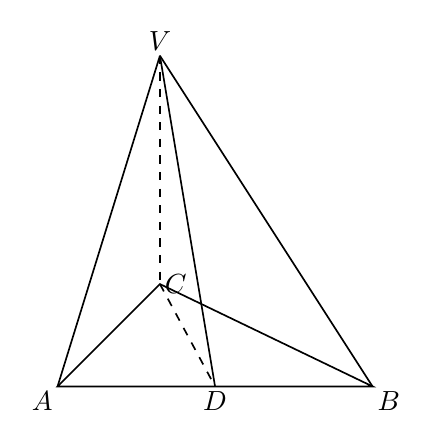
\begin{tikzpicture}[scale=1.0, semithick,
  every node/.style={inner sep=1.5pt}]
  \coordinate (A) at (0,0);
  \coordinate (B) at (4.0,0);
  \coordinate (C) at (1.3,1.3);
  \coordinate (V) at (1.3,4.2);
  \coordinate (D) at (2.0,0);

  \draw (A) -- (B) -- (C) -- cycle;
  \draw (V) -- (A);
  \draw (V) -- (B);
  \draw[dashed] (V) -- (C);
  \draw (V) -- (D);
  \draw[dashed] (C) -- (D);

  \node[below left] at (A) {$A$};
  \node[below right] at (B) {$B$};
  \node[right] at (C) {$C$};
  \node[above] at (V) {$V$};
  \node[below] at (D) {$D$};
\end{tikzpicture}
\end{center}
\nopagebreak[4]
\Needspace{4\baselineskip}
\textbf{解析}

\Needspace{5\baselineskip}
以 $C$ 为原点，$CA$，$CB$，$CV$ 为 $x$，$y$，$z$ 轴：

\nopagebreak[4]
\[C(0,0,0),\ A(a,0,0),\ B(0,a,0),\ D\left(\frac a2,\frac a2,0\right),\ V(0,0,h).\]

（1）$\overrightarrow{AB}=(-a,a,0)$，$\overrightarrow{CD}=\left(\dfrac a2,\dfrac a2,0\right)$，点积为 $0$，故 $AB\perp CD$。又 $VC\perp$ 底面，故 $VC\perp AB$。于是 $AB\perp$ 平面 $VCD$，从而平面 $VAB\perp$ 平面 $VCD$。

\Needspace{5\baselineskip}
（2）$\overrightarrow{BC}=(0,-a,0)$。平面 $VAB$ 的法向量

\nopagebreak[4]
\[\boldsymbol n=\overrightarrow{VA}\times\overrightarrow{VB}=(ah,ah,a^2)\sim(h,h,a).\]

\Needspace{5\baselineskip}
设 $BC$ 与平面所成角为 $\varphi$，则

\nopagebreak[4]
\[\sin\varphi=\frac{|\overrightarrow{BC}\cdot\boldsymbol n|}{|\overrightarrow{BC}||\boldsymbol n|}
=\frac{ah}{a\sqrt{2h^2+a^2}}=\frac{h}{\sqrt{2h^2+a^2}}.\]

\Needspace{5\baselineskip}
由 $\varphi=\dfrac{\pi}{6}$ 得

\nopagebreak[4]
\[\frac{h^2}{2h^2+a^2}=\frac14\ \Rightarrow\ 2h^2=a^2\ \Rightarrow\ h=\frac a{\sqrt2}.\]

\Needspace{5\baselineskip}
又 $CD=\dfrac{a\sqrt2}{2}$，故

\nopagebreak[4]
\[\tan\theta=\frac{VC}{CD}=\frac{h}{a\sqrt2/2}=1,\]

\nopagebreak[4]
\[\theta=\frac{\pi}{4}.\]

\gkanswer{答案：（1）证明见解析；（2）$\theta=\dfrac{\pi}{4}$。}

\end{answer}
\begin{answer}
\gksolhead{18}{}

\textbf{题目}：

某商品每件成本 $9$ 元，售价 $30$ 元，每星期卖出 $432$ 件。如果降低价格，销售量可以增加，且每星期多卖出的商品件数与商品单价的降低值 $x$（单位：元，$0\leqslant x\leqslant30$）的平方成正比。已知商品单价降低 $2$ 元时，一星期多卖出 $24$ 件。

（1）将一个星期的商品销售利润表示成 $x$ 的函数；

（2）如何定价才能使一个星期的商品销售利润最大？

\Needspace{4\baselineskip}
\textbf{解析}

\Needspace{5\baselineskip}
（1）设多卖出 $kx^2$ 件。$x=2$ 时多卖 $24$ 件：

\nopagebreak[4]
\[4k=24\ \Rightarrow\ k=6.\]

\Needspace{5\baselineskip}
每件利润 $30-x-9=21-x$，故

\nopagebreak[4]
\[P(x)=(21-x)(432+6x^2),\quad0\leqslant x\leqslant30.\]

\Needspace{5\baselineskip}
（2）展开：

\nopagebreak[4]
\[P(x)=-6x^3+126x^2-432x+9072,\]

\nopagebreak[4]
\[P'(x)=-18x^2+252x-432=-18(x-2)(x-12).\]

\Needspace{5\baselineskip}
$0<x<2$ 时 $P'<0$，$2<x<12$ 时 $P'>0$，$x>12$ 时 $P'<0$，故 $x=12$ 时利润最大。定价

\nopagebreak[4]
\[30-12=18\ \text{\text{元}},\]

\Needspace{5\baselineskip}
最大利润

\nopagebreak[4]
\[P(12)=9\times(432+864)=11664\ \text{\text{元}}.\]

\gkanswer{答案：（1）$P(x)=(21-x)(432+6x^2)$，$0\leqslant x\leqslant30$；（2）定价 $18$ 元，最大利润 $11664$ 元。}

\end{answer}
\begin{answer}
\gksolhead{19}{}

\textbf{题目}：

设二次函数 $f(x)=x^2+ax+a$，方程 $f(x)-x=0$ 的两根 $x_1$ 和 $x_2$ 满足 $0<x_1<x_2<1$。

（1）求实数 $a$ 的取值范围；

（2）试比较 $f(0)f(1)-f(0)$ 与 $\dfrac1{16}$ 的大小，并说明理由。

\Needspace{4\baselineskip}
\textbf{解析}

\Needspace{5\baselineskip}
（1）方程 $f(x)-x=0$ 即

\nopagebreak[4]
\[g(x)=x^2+(a-1)x+a=0.\]

\Needspace{5\baselineskip}
两根在 $(0,1)$ 内，需

\nopagebreak[4]
\[g(0)=a>0,\qquad g(1)=2a>0,\]

\Needspace{5\baselineskip}
对称轴 $x=\dfrac{1-a}{2}\in(0,1)$，即 $-1<a<1$，且判别式

\nopagebreak[4]
\[\Delta=(a-1)^2-4a=a^2-6a+1>0.\]

\Needspace{5\baselineskip}
解得 $a<3-2\sqrt2$ 或 $a>3+2\sqrt2$。结合 $0<a<1$，得

\nopagebreak[4]
\[0<a<3-2\sqrt2.\]

\Needspace{5\baselineskip}
（2）$f(0)=a$，$f(1)=1+2a$，故

\nopagebreak[4]
\[f(0)f(1)-f(0)=a(1+2a)-a=2a^2.\]

\Needspace{5\baselineskip}
由（1），$a<3-2\sqrt2$。又

\nopagebreak[4]
\[3-2\sqrt2=\frac1{3+2\sqrt2}<\frac{\sqrt2}{8},\]

\Needspace{5\baselineskip}
故

\nopagebreak[4]
\[2a^2<2\left(\frac{\sqrt2}{8}\right)^2=\frac1{16}.\]

\gkanswer{答案：（1）$0<a<3-2\sqrt2$；（2）$f(0)f(1)-f(0)<\dfrac1{16}$。}

\end{answer}
\begin{answer}
\gksolhead{20}{}

\textbf{题目}：

已知数列 $\{a_n\}$ 和 $\{b_n\}$ 满足：$a_1=1$，$a_2=2$，$a_n>0$，$b_n=\sqrt{a_na_{n+1}}$（$n\in\mathbf N^*$），且 $\{b_n\}$ 是以 $q$ 为公比的等比数列。

（1）证明：$a_{n+2}=a_nq^2$；

（2）若 $c_n=a_{2n-1}+2a_{2n}$，证明数列 $\{c_n\}$ 是等比数列；

（3）求和：$\dfrac1{a_1}+\dfrac1{a_2}+\dfrac1{a_3}+\dfrac1{a_4}+\cdots+\dfrac1{a_{2n-1}}+\dfrac1{a_{2n}}$。

\Needspace{4\baselineskip}
\textbf{解析}

\Needspace{5\baselineskip}
（1）由 $\{b_n\}$ 公比为 $q$，

\nopagebreak[4]
\[\frac{b_{n+1}}{b_n}=q\ \Rightarrow\ \frac{\sqrt{a_{n+1}a_{n+2}}}{\sqrt{a_na_{n+1}}}=q,\]

\nopagebreak[4]
\[\sqrt{\frac{a_{n+2}}{a_n}}=q\ \Rightarrow\ a_{n+2}=a_nq^2.\]

\Needspace{5\baselineskip}
（2）由（1），奇数项与偶数项分别成公比 $q^2$ 的等比数列：

\nopagebreak[4]
\[a_{2n-1}=q^{2n-2},\qquad a_{2n}=2q^{2n-2}.\]

\Needspace{5\baselineskip}
故

\nopagebreak[4]
\[c_n=a_{2n-1}+2a_{2n}=5q^{2n-2},\]

是公比为 $q^2$ 的等比数列。

\Needspace{5\baselineskip}
（3）奇数项倒数之和

\nopagebreak[4]
\[\sum_{k=1}^n q^{-2(k-1)}=\frac{1-q^{-2n}}{1-q^{-2}},\]

\Needspace{5\baselineskip}
偶数项倒数之和

\nopagebreak[4]
\[\sum_{k=1}^n\frac1{2q^{2(k-1)}}=\frac12\cdot\frac{1-q^{-2n}}{1-q^{-2}}.\]

\Needspace{5\baselineskip}
合计

\nopagebreak[4]
\[\frac32\cdot\frac{1-q^{-2n}}{1-q^{-2}}\quad(q\neq1).\]

$q=1$ 时每项倒数为 $1$ 或 $\dfrac12$，和为 $\dfrac{3n}2$。

\gkanswer{答案：（1）（2）证明见解析；（3）$\dfrac32\cdot\dfrac{1-q^{-2n}}{1-q^{-2}}$（$q\neq1$），$q=1$ 时为 $\dfrac{3n}2$。}

\end{answer}
\begin{answer}
\gksolhead{21}{}

\textbf{题目}：

在平面直角坐标系 $xOy$ 中，过定点 $C(0,p)$ 作直线与抛物线 $x^2=2py$（$p>0$）相交于 $A$，$B$ 两点。

（1）若点 $N$ 是点 $C$ 关于坐标原点 $O$ 的对称点，求 $\triangle ANB$ 面积的最小值；

（2）是否存在垂直于 $y$ 轴的直线 $l$，使得 $l$ 被以 $AC$ 为直径的圆截得的弦长恒为定值？若存在，求出 $l$ 的方程；若不存在，说明理由。
\nopagebreak[4]
\begin{center}% 2007 年湖北卷文科第 21 题：抛物线 x^2=2py，过 C(0,p) 的直线交于 A、B，
%   N 为 C 关于原点的对称点。
% 来源 PDF：gaokaomath-src/普通高考/2007/2007湖北文.pdf
% SHA-256：290a153da24ec0f3a3abb8bb916d9b7e06d203d3ef5bd7bb221c93f7f1b1cacb
% 原页：2007湖北文.pdf 第 2 页（A3 三栏）第 3 栏，书页码 378。
% 重绘依据：按原页抛物线、割线与 C、N 的位置重绘，p=1 仅作示意。
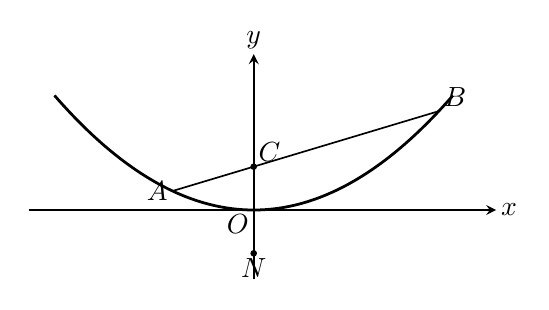
\begin{tikzpicture}[x=1.1cm, y=0.55cm, semithick,
  every node/.style={inner sep=1.5pt}]
  \draw[->,>=stealth] (-2.6,0) -- (2.8,0) node[right] {$x$};
  \draw[->,>=stealth] (0,-1.6) -- (0,3.6) node[above] {$y$};
  \node[below left] at (0,0) {$O$};

  \draw[domain=-2.3:2.3,samples=120,line width=1pt] plot (\x,{\x*\x/2});

  \coordinate (C) at (0,1);
  \coordinate (N) at (0,-1);
  \coordinate (A) at (-0.937,0.439);
  \coordinate (B) at (2.137,2.283);

  \draw (A) -- (B);
  \fill (C) circle (1.2pt);
  \fill (N) circle (1.2pt);
  \node[above right] at (C) {$C$};
  \node[below] at (N) {$N$};
  \node[left] at (A) {$A$};
  \node[above right] at (B) {$B$};
\end{tikzpicture}
\end{center}
\nopagebreak[4]
\Needspace{4\baselineskip}
\textbf{解析}

\Needspace{5\baselineskip}
（1）设直线 $y=kx+p$，代入 $x^2=2py$：

\nopagebreak[4]
\[x^2-2pkx-2p^2=0.\]

\Needspace{5\baselineskip}
设 $A(x_1,y_1)$，$B(x_2,y_2)$，则

\nopagebreak[4]
\[x_1+x_2=2pk,\qquad x_1x_2=-2p^2.\]

\Needspace{5\baselineskip}
$N(0,-p)$，面积

\nopagebreak[4]
\[S_{\triangle ANB}=\frac12|x_1(y_2+p)-x_2(y_1+p)|.\]

\Needspace{5\baselineskip}
计算得

\nopagebreak[4]
\[S=p|x_2-x_1|=p\sqrt{(2pk)^2+8p^2}=2p^2\sqrt{k^2+2}\geqslant2\sqrt2p^2,\]

等号当 $k=0$。

\Needspace{5\baselineskip}
（2）以 $AC$ 为直径的圆圆心为 $\left(\dfrac{x_1}2,\dfrac{y_1+p}2\right)$，半径平方

\nopagebreak[4]
\[r^2=\frac{x_1^2+(y_1-p)^2}{4}.\]

\Needspace{5\baselineskip}
设 $l:y=m$，弦长平方

\nopagebreak[4]
\[\ell^2=4\left[r^2-\left(m-\frac{y_1+p}{2}\right)^2\right]
=x_1^2+(y_1-p)^2-(2m-y_1-p)^2.\]

\Needspace{5\baselineskip}
利用 $x_1^2=2py_1$ 化简：

\nopagebreak[4]
\[\ell^2=(4m-2p)y_1+4mp-4m^2.\]

\Needspace{5\baselineskip}
要使 $\ell$ 与 $y_1$ 无关，需

\nopagebreak[4]
\[4m-2p=0\ \Rightarrow\ m=\frac p2.\]

\Needspace{5\baselineskip}
此时

\nopagebreak[4]
\[\ell^2=p^2,\]

\Needspace{5\baselineskip}
弦长恒为 $p$。故存在直线

\nopagebreak[4]
\[l:\ y=\frac p2.\]

\gkanswer{答案：（1）$2\sqrt2p^2$；（2）存在，$l:y=\dfrac p2$。}

\end{answer}